

\chapter{Using SimHPN}

\section{Short description of the GUI}
The $SimHPN$ simulator supports {\color{red} infinite server} and {\color{red}product server semantics} for both discrete and continuous transitions. Moreover, deterministic delays with single server semantics are also supported for discrete transitions. Both the data related to the model description, i.e., net structure, initial marking and timing parameter, and the output results, i.e., time trajectories, are MATLAB variables. At the end of the simulation, the user can export the data to the MATLAB workspace where can be used for further analysis. 

The $SimHPN$ toolbox (\url{http://webdiis.unizar.es/GISED/?q=tool/simhpn}) provides a Graphical User Interface (GUI) that enables the user to easily perform simulations and carry out analysis methods.  This GUI consists of a MATLAB figure window, exhibiting a \emph{Menu bar} and three control panels: 
\begin{itemize}
\item[(i)] \emph{Drawing Area}, 
\item[(ii)] \emph{Options panel}, and 
\item[(iii)] \emph{Model Management panel}. 
\end{itemize}
Fig. \ref{GUI} presents a hard-copy screenshot of the main window opened by $SimHPN$ toolbox, where all the component parts of the GUI are visible.

\begin{figure*}[!htb]
   \centering{
   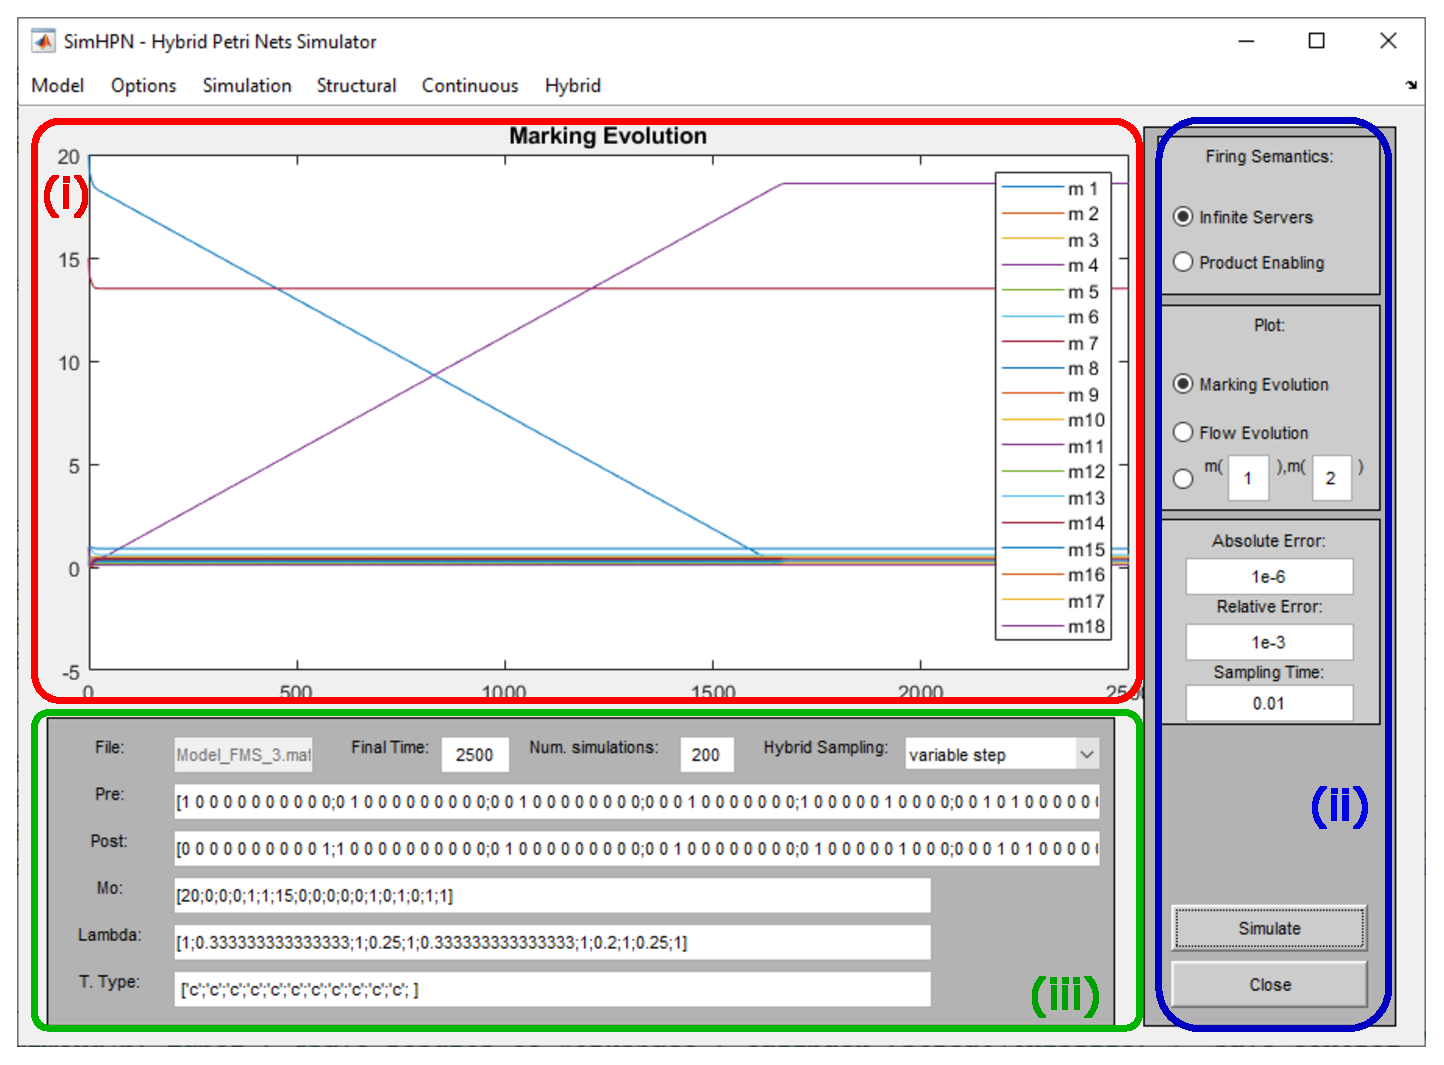
\includegraphics[width=.85\textwidth]{figs/MainWindowSimHPN.eps}}
   \caption[htb!]{Sketch of the main window of $SimHPN$}\label{GUI}
\end{figure*}

The \emph{Menu bar} (placed horizontally, on the top of the window in Fig. \ref{GUI}) displays a set of six drop-down menus at the top of the window, where the user can select different features available in the $SimHPN$ toolbox. These menus are: \emph{Model}, \emph{Options}, \emph{Simulation}, \emph{Structural}, \emph{Continuous} and \emph{Hybrid}.

The {\color{blue}\emph{Model menu}} contains the pop-up menus:
\begin{itemize}
\item \emph{Import from Pmeditor}, 
\item \emph{Import from TimeNet} and 
\item \emph{Import from .mat file} 
\item \emph{Save to .mat file}
\end{itemize}
that implement several importing options for the matrices, $\b{Pre}$, $\b{Post}$, $\mo$, etc, that describe the net system. Such matrices can be introduced manually or through two Petri nets editors: PMEditeur and TimeNet \cite{IPZiKn95}.  Moreover, the matrices can be automatically loaded from a $.mat$ file (MATLAB file format) or loaded from variables defined in the workspace, this is done just by writing the name of the variable to be used in the corresponding edit boxes. 

If the model is imported from a $.mat$ file, the following variables should be defined in the $.mat$ file:

\begin{itemize}
\item $Pre$ - is a $|P| \times$ $|T|$ matrix containing the weight of the arcs from places to transitions;
\item $Post$ - is a $|P| \times$ $|T|$   containing the weight of the arcs from transitions to places;
\item $M0$ - is a column vector of dimension $|P|$ containing the initial marking;
\item $Lambda$ - is a column vector of dimension $|T|$ containing the firing rates of transitions:
\item $Trans\_Type$ - is a column vector of dimension $|T|$ containing the type of transitions. Each element can have one of the following values:
\begin{itemize}
\item $'c'$ - for continuous transition;
\item $'d'$ - for stochastic discrete transitions;
\item $'q'$ -  for deterministic  discrete transitions.
\end{itemize}
\end{itemize}


The last option (i.e., \emph{Save to .mat file}) saves to a .mat file the matrices already defined in the edit boxes of $SimHPN$.

The {\color{blue}\emph{Options}} menu contains only the pop-up menu 
\begin{itemize}
\item \emph{Show Figure Toolbar} 
\end{itemize}
that allows to show the characteristic toolbar of the MATAB figure object that permits, for example, the use of zoom tool on the displayed graphic in the \emph{Drawing Area}.

The {\color{blue}\emph{Simulation menu}} contains the pop-up menus: 
\begin{itemize}
\item \emph{Markings to plot}, 
\item \emph{Flows to plot}, and 
\item \emph{Save results to workspace}. 
\end{itemize}
The pop-up menus \emph{Markings to plot}, \emph{Flows to plot} allow the user to select the components of marking vector and flow vector that will be plotted after  simulation in the \emph{Drawing area}. The pop-up menu \emph{Save results to workspace}  permits to export, after simulation, the marking and flow evolution to variables in the MATLAB workspace.

The rest of the menus call procedures for analysis and synthesis of PN model if it is assumed discrete Petri net (\emph{Structural} menu), fully continuous Petri net (\emph{Continuous} menu), and Hybrid Petri net (\emph{Hybrid} menu). The different functions of these menus will be further explained in the following sections.


The \emph{Drawing area} (located in the left and central side of the window in Fig. \ref{GUI}), is a MATLAB axes object where the trajectories of the simulation results are plotted. The components of markings and flows that will be represented are selected from the menu.

The \emph{Options panel} (placed, as a horizontal bar, on the right part of the window Fig. \ref{GUI}) presents a number of options related to the model. From top to bottom: (a) two radio buttons to select the firing semantics for continuous and discrete exponential  transitions; (b) three radio buttons allowing to select the variables to be plotted in the \emph{Drawing Area}, the simulator allows one to plot the evolution of the marking
of the places, the evolution of the flow of the transitions and
the evolution of the marking of one place vs. the marking of other
place; (c) three edit boxes to fix the maximum absolute and relative errors allowed by the simulated trajectory and the sampling time used in simulations (see next subsection for more details on the selection of the sampling time); (d) a \emph{Simulate} button to start a new simulation; (e) a \emph{Compute Bounds} button that computes performance bounds for continuous nets under infinite server semantics; (f) a \emph{P T semiflows} button to compute the minimal P- and T-semiflows of the net, the results are displayed on the MATLAB command window and can be used for future analysis tasks; and (g) a \emph{Close} button to close the $SimHPN$ toolbox.

The \emph{Model Management Panel} panel is composed of different edit boxes (placed in the bottom left corner of the window in Fig. \ref{GUI}), where the $SimHPN$ toolbox displays the current values of the matrices describing the net system and permits to select the simulation time and the number of simulations to be performed (this last parameter is ignored if the net contains no stochastic transitions).  The required matrices for a system in order to be simulated are: $\b{Pre}$ and $\b{Post}$ matrices, initial marking $\mo$, the parameter $\b{\lambda}$ of each transition, and the type of each transition. This last parameter is equal to 'c' for continuous transitions, to 'd' for stochastic discrete transitions and to 'q' for deterministic discrete transitions. Notice that if the type of a transition is 'q' then single server semantics is adopted for its firing and therefore the selection of firing semantics in the \emph{Options panel} will be ignored for this transition.

\section{Analysis and design tools}

In the following, we describe the different analysis and design tools implemented in SimHPN. 

The {\color{blue}\emph{Structural menu}} contains different analysis techniques to compute the following properties of a given net structure:

\begin{itemize}
\item \emph{Conservativeness}: Test if the net structure is conservative and computes its different conservative components.
\item \emph{Consistency}: Test if the net structure is consistent and computes its different repetitive components.
\item \emph{P T semiflows}: Compute the T-semiflows and P-semiflows of the net structure, and gives you the option to save the solutions to the workspace.
\end{itemize} 


The {\color{blue}\emph{Continuous menu}} contains different analysis and design tools developed for continuous and timed continuous PN systems. In the following, the different implemented methods are detailed. 

The \emph{Compute bounds} menu provide algorithms that compute lower and upper bound for infinite servers semantics and upper bound for finite servers semantics for the case of \emph{unforced} systems (with no control). Based on the methods developped in \cite{julvez2005steady}. It is only valid for mono-t-semiflow systems. 

The \emph{Optimal} submenu contains the pop-up menus \emph{Optimal Observability} and \emph{Optimal Control}. Such pop-up menus perform calls to the algorithms for computing optimal steady state for the \emph{forced} case (with control) \cite{mahulea2008steady} and optimal sensor placement for continuous Petri nets with infinite server semantics.

There are different submenus that contain different algorithms for the implementation of \emph{control laws}, permitting the system to reach a desired final marking if the net is continuous under infinite server semantics. 

After using a particular control law, it is possible to use the menu \emph{Save results to workspace} to save the computed input and the marking trajectory of the forced system. Between the implemented algorithms are different ON/OFF Methods \cite{ONOFFmethodsWANG2014}, Affine control laws \cite{AffineLawThesisRenato}, minimum-time control law \cite{ApproachingMinTimeAPAYDINOZKAN2011}, \cite{minTime}, minimum-time control flow \cite{MinTimeControlCF}. See the cited references for the particular pre-requisites of each method.

The menus for Structural controllability analysis and Diagnosis are explained with more detail in the following sections.

\subsection{Structural controllability analysis}

This submenu provides a set of algorithms that have been specifically implemented for the structural controllability analysis of timed continuous Petri nets \cite{arzola2023structural}. These algorithms offer various tests for determining the net rank-controllability property of a given TCPN and the computation of the sets of equilibrium markings of the system.

In a live and bounded TCPN system, the concept of net rank-controllability serves as a sufficient condition for determining whether the system is controllable over its connected equilibrium sets. See Section 5.4 for examples and more details on the application of these tools.



\subsubsection{Influence of controllable transitions}

This routine computes the sets of \emph{influenced places and transitions by the controllable transitions}, $P_{I}$ and $T_{I}$. This is a necessary condition for net rank-controllability and it indicates the sets of nodes whose marking and flow can be affected by the activity on the controllable transitions, regardless of the configuration. If a controllable transition does not influence all places in the net, the net cannot be net rank-controllable. It is carried out by implementing Algorithm 1 in \cite{arzola2023structural}. 

When the user selects this routine, a window is opened and the user should introduce the set of controllable transitions. After this, the results are shown in a pop-up window containing one of two possible messages:  1) A message indicating that influence is not total and indicating the sets of influenced nodes, $P_I\subset P$ and $T_I\subset T$, 2) A message indicating that influence is total, i.e., $P_I=P$ and $T_I=T$.


\subsubsection{Net rank-controllability test}


This routine verifies sufficient conditions for net rank-controllability. It is carried out by implementing Algorithm 2 in \cite{arzola2023structural}. It is efficiently performed by verifying some structural conditions:\\
$\bullet$ \textbf{Structural Condition 1 (SC1)}: Given $\mathcal{N}$, the influence of $T_c$ is total.\\
$ \bullet$ \textbf{Structural Condition 2 (SC2)}: Given $\mathcal{N}$, for all choice place, $p_c\in \{p\in P | |p^{\bullet}|>1\}$, $p_c^\bullet\subseteq T_{c}$.\\
$ \bullet$ \textbf{Structural Condition 3 (SC3)}: Given $\mathcal{N}$, let $T_F = \{t\in T| |t^{\bullet}|>1\}$ be the set of fork transitions. For all $t_f\in T_F$, we assume that $| \{t_f^\bullet\}^\bullet\cap T_{nc}|\leq 1$.\\

When the user selects this routine, a window is opened and the user should introduce the set of controllable transitions. After this, the results are shown in a pop-up window indicating if the net fulfills the property. In case it is not fulfilled, it indicates which one of the structural conditions does not hold.


\subsubsection{Equilibrium connectivity graph}

This routine computes the equilibrium sets and their connectivity for a specified TCPN system. The output is a graph where each node represents a configuration of the system whose region contains equilibrium markings, and the edges indicate the connection between the equilibrium markings of the different regions. You can save the results of this analysis by selecting the "Save Equilibrium Connectivity Graph to Workspace" submenu. Additionally, if all the equilibrium sets are connected, the function will return a message indicating this.
\subsection{Diagnosis}


The \emph{Diagnosis} submenu calls the algorithms that perform fault diagnosis for untimed continuous Petri nets \cite{ARMASECASI12}. Once the user selects this option, a window as in Fig.~\ref{fig:diag} is opened and the user should introduce the input parameters:
\begin{enumerate}
\item The number of observable transitions. Without loss of generality, it is assumed that the first transitions are observable and the rest are unobservable.
\item The firing sequence of observable transitions.
\item The firing amount of each transition of the firing sequence.
\item Number of fault classes.
\end{enumerate}


\begin{figure*}[!htb]
   \centering{
   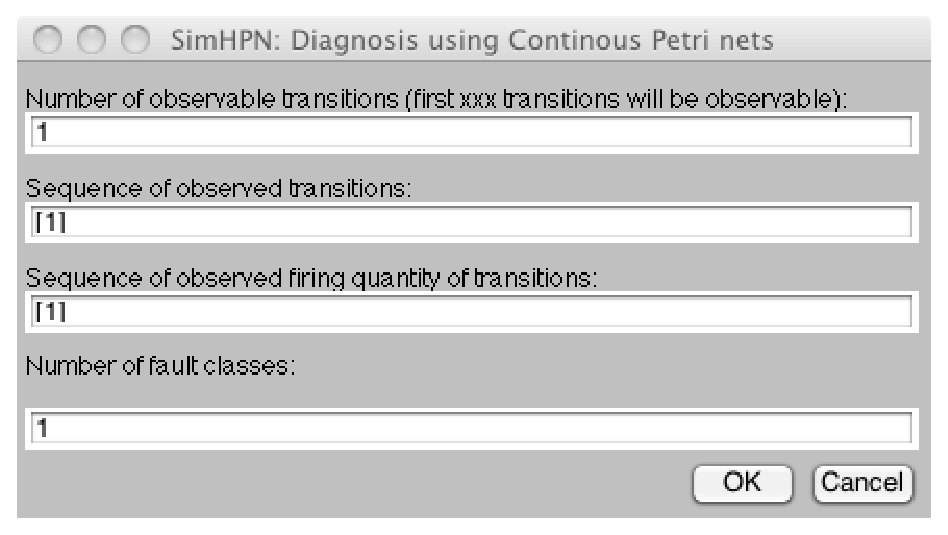
\includegraphics[width=.85\textwidth]{figs/diag1.eps}}
   \caption[htb!]{Sketch of the uicontrols for the diagnosis.}\label{fig:diag}
\end{figure*}

After this, an uicontrol will be used to introduce the transitions belonging to each fault class. All the results are shown at the MATLAB command prompt. See Section~\ref{sec:fdsexamps} for examples and more details on the parameters for fault detection.


\section{Script simulation}
$SimHPN$ permits the simulation of a hybrid Petri net from the MATLAB prompt, without open the GUI. This is useful if one wants to implement a script and simulate a hybrid Petri net for some particular input parameters. This can be done in two different ways depending on the type of the input model.

\textbf{Continuous Petri net}. If the net has only continuous transitions, the following command can be used for its simulation:

\begin{verbatim}
[m,f,t] = SimHPN_Simul(Pre, Post, m0, tf, lambda, seman, erel, eabs);
\end{verbatim}
where, 
\begin{itemize}
\item $Pre$ - is a $|P| \times$ $|T|$ matrix containing the weight of the arcs from places to transitions;
\item $Post$ - is a $|P| \times$ $|T|$   containing the weight of the arcs from transitions to places;
\item $m0$ - is a column vector of dimension $|P|$ containing the initial marking;
\item $tf$ - is the final time for simulation;
\item $lambda$ - is a column vector of dimension $|T|$ containing the firing rates of transitions:
\item $seman = 1$ - if transitions are with infinite server semantics and $seman = 2$ - if product firing semantics is considered for transitions;
\item $erel$ - relative error;
\item $eabs$ - absolute error.
\end{itemize}

The returned parameters are:

\begin{itemize}
\item $m$ - a matrix of dimension $|t| \times |P|$ is the matrix defining the marking evolutions;
\item $f$ - a matrix of dimension $|t| \times |T|$ is the matrix defining the flow evolutions;
\item $t$ - a row vector containing the time instants for which the markings and the flows are defined.
\end{itemize}

\textbf{Hybrid Petri net}. If the net is not purely continuous, function \emph{SimHPN\_SimHyb} 
should be used. This function is defined as follows:

\begin{verbatim}
[m,f,t] = SimHPN_SimHyb(Pre,Post,lambda,type,m0,nsim,tsim,seman,mode,delta)
\end{verbatim}

The input parameters are:

\begin{itemize}
\item $Pre$ - is a $|P| \times$ $|T|$ matrix containing the weight of the arcs from places to transitions;
\item $Post$ - is a $|P| \times$ $|T|$   containing the weight of the arcs from transitions to places;
\item $lambda$ - is a column vector of dimension $|T|$ containing the firing rates of transitions:
\item $type$ - is a column vector of dimension $|T|$ containing the type of transitions. Each element can have one of the following values:
\begin{itemize}
\item $'c'$ - for continuous transition;
\item $'d'$ - for stochastic discrete transitions;
\item $'q'$ -  for deterministic  discrete transitions.
\end{itemize}
\item $m0$ - is a column vector of dimension $|P|$ containing the initial marking;
\item $nsim$ - number of simulations especially useful for stochastic transitions;
\item $tsim$ - simulation time
\item $seman = 1$ - if continuous transitions are with infinite server semantics and $seman = 2$ is product firing semantics is considered for continuous transitions;
\item $mode = 1$ - if constant hybrid sampling step will be used;  $mode = 2$ - if variable hybrid sampling step will be used;  
\item $delta$ - sampling timed used in the case of $mode = 1$.
\end{itemize}
 
 After a simulation, the returned parameters are:

\begin{itemize} 
\item $m$ - a matrix of dimension $|t| \times |P|$ is the matrix defining the marking evolutions;
\item $f$ - a matrix of dimension $|t| \times |T|$ is the matrix defining the flow evolutions;
\item $t$ - a row vector containing the time instants for which the markings and the flows are defined.
\end{itemize}

\newpage

